\documentclass[11pt,a4paper]{report}
\usepackage[textwidth=37em,vmargin=30mm]{geometry}
\usepackage{calc,xunicode,amsmath,amssymb,paralist,enumitem,tabu,booktabs,datetime2,xeCJK,xeCJKfntef,listings}
\usepackage{tocloft,fancyhdr,tcolorbox,xcolor,graphicx,eso-pic,xltxtra,xelatexemoji}

\newcommand{\envyear}[0]{2024}
\newcommand{\envdatestr}[0]{2024-11-03}
\newcommand{\envfinaldir}[0]{webdb/2024/20241103/final}

\usepackage[hidelinks]{hyperref}
\hypersetup{
    colorlinks=false,
    pdfpagemode=FullScreen,
    pdftitle={Web Digest - \envdatestr}
}

\setlength{\cftbeforechapskip}{10pt}
\renewcommand{\cftchapfont}{\rmfamily\bfseries\large\raggedright}
\setlength{\cftbeforesecskip}{2pt}
\renewcommand{\cftsecfont}{\sffamily\small\raggedright}

\setdefaultleftmargin{2em}{2em}{1em}{1em}{1em}{1em}

\usepackage{xeCJK,xeCJKfntef}
\xeCJKsetup{PunctStyle=plain,RubberPunctSkip=false,CJKglue=\strut\hskip 0pt plus 0.1em minus 0.05em,CJKecglue=\strut\hskip 0.22em plus 0.2em}
\XeTeXlinebreaklocale "zh"
\XeTeXlinebreakskip = 0pt


\setmainfont{Brygada 1918}
\setromanfont{Brygada 1918}
\setsansfont{IBM Plex Sans}
\setmonofont{JetBrains Mono NL}
\setCJKmainfont{Noto Serif CJK SC}
\setCJKromanfont{Noto Serif CJK SC}
\setCJKsansfont{Noto Sans CJK SC}
\setCJKmonofont{Noto Sans CJK SC}

\setlength{\parindent}{0pt}
\setlength{\parskip}{8pt}
\linespread{1.15}

\lstset{
	basicstyle=\ttfamily\footnotesize,
	numbersep=5pt,
	backgroundcolor=\color{black!5},
	showspaces=false,
	showstringspaces=false,
	showtabs=false,
	tabsize=2,
	captionpos=b,
	breaklines=true,
	breakatwhitespace=true,
	breakautoindent=true,
	linewidth=\textwidth
}






\newcommand{\coverpic}[2]{
    % argv: itemurl, authorname
    Cover photo by #2~~(\href{#1}{#1})
}
\newcommand{\makeheader}[0]{
    \begin{titlepage}
        % \newgeometry{hmargin=15mm,tmargin=21mm,bmargin=12mm}
        \begin{center}
            
            \rmfamily\scshape
            \fontspec{BaskervilleF}
            \fontspec{Old Standard}
            \fontsize{59pt}{70pt}\selectfont
            WEB\hfill DIGEST
            
            \vfill
            % \vskip 30pt
            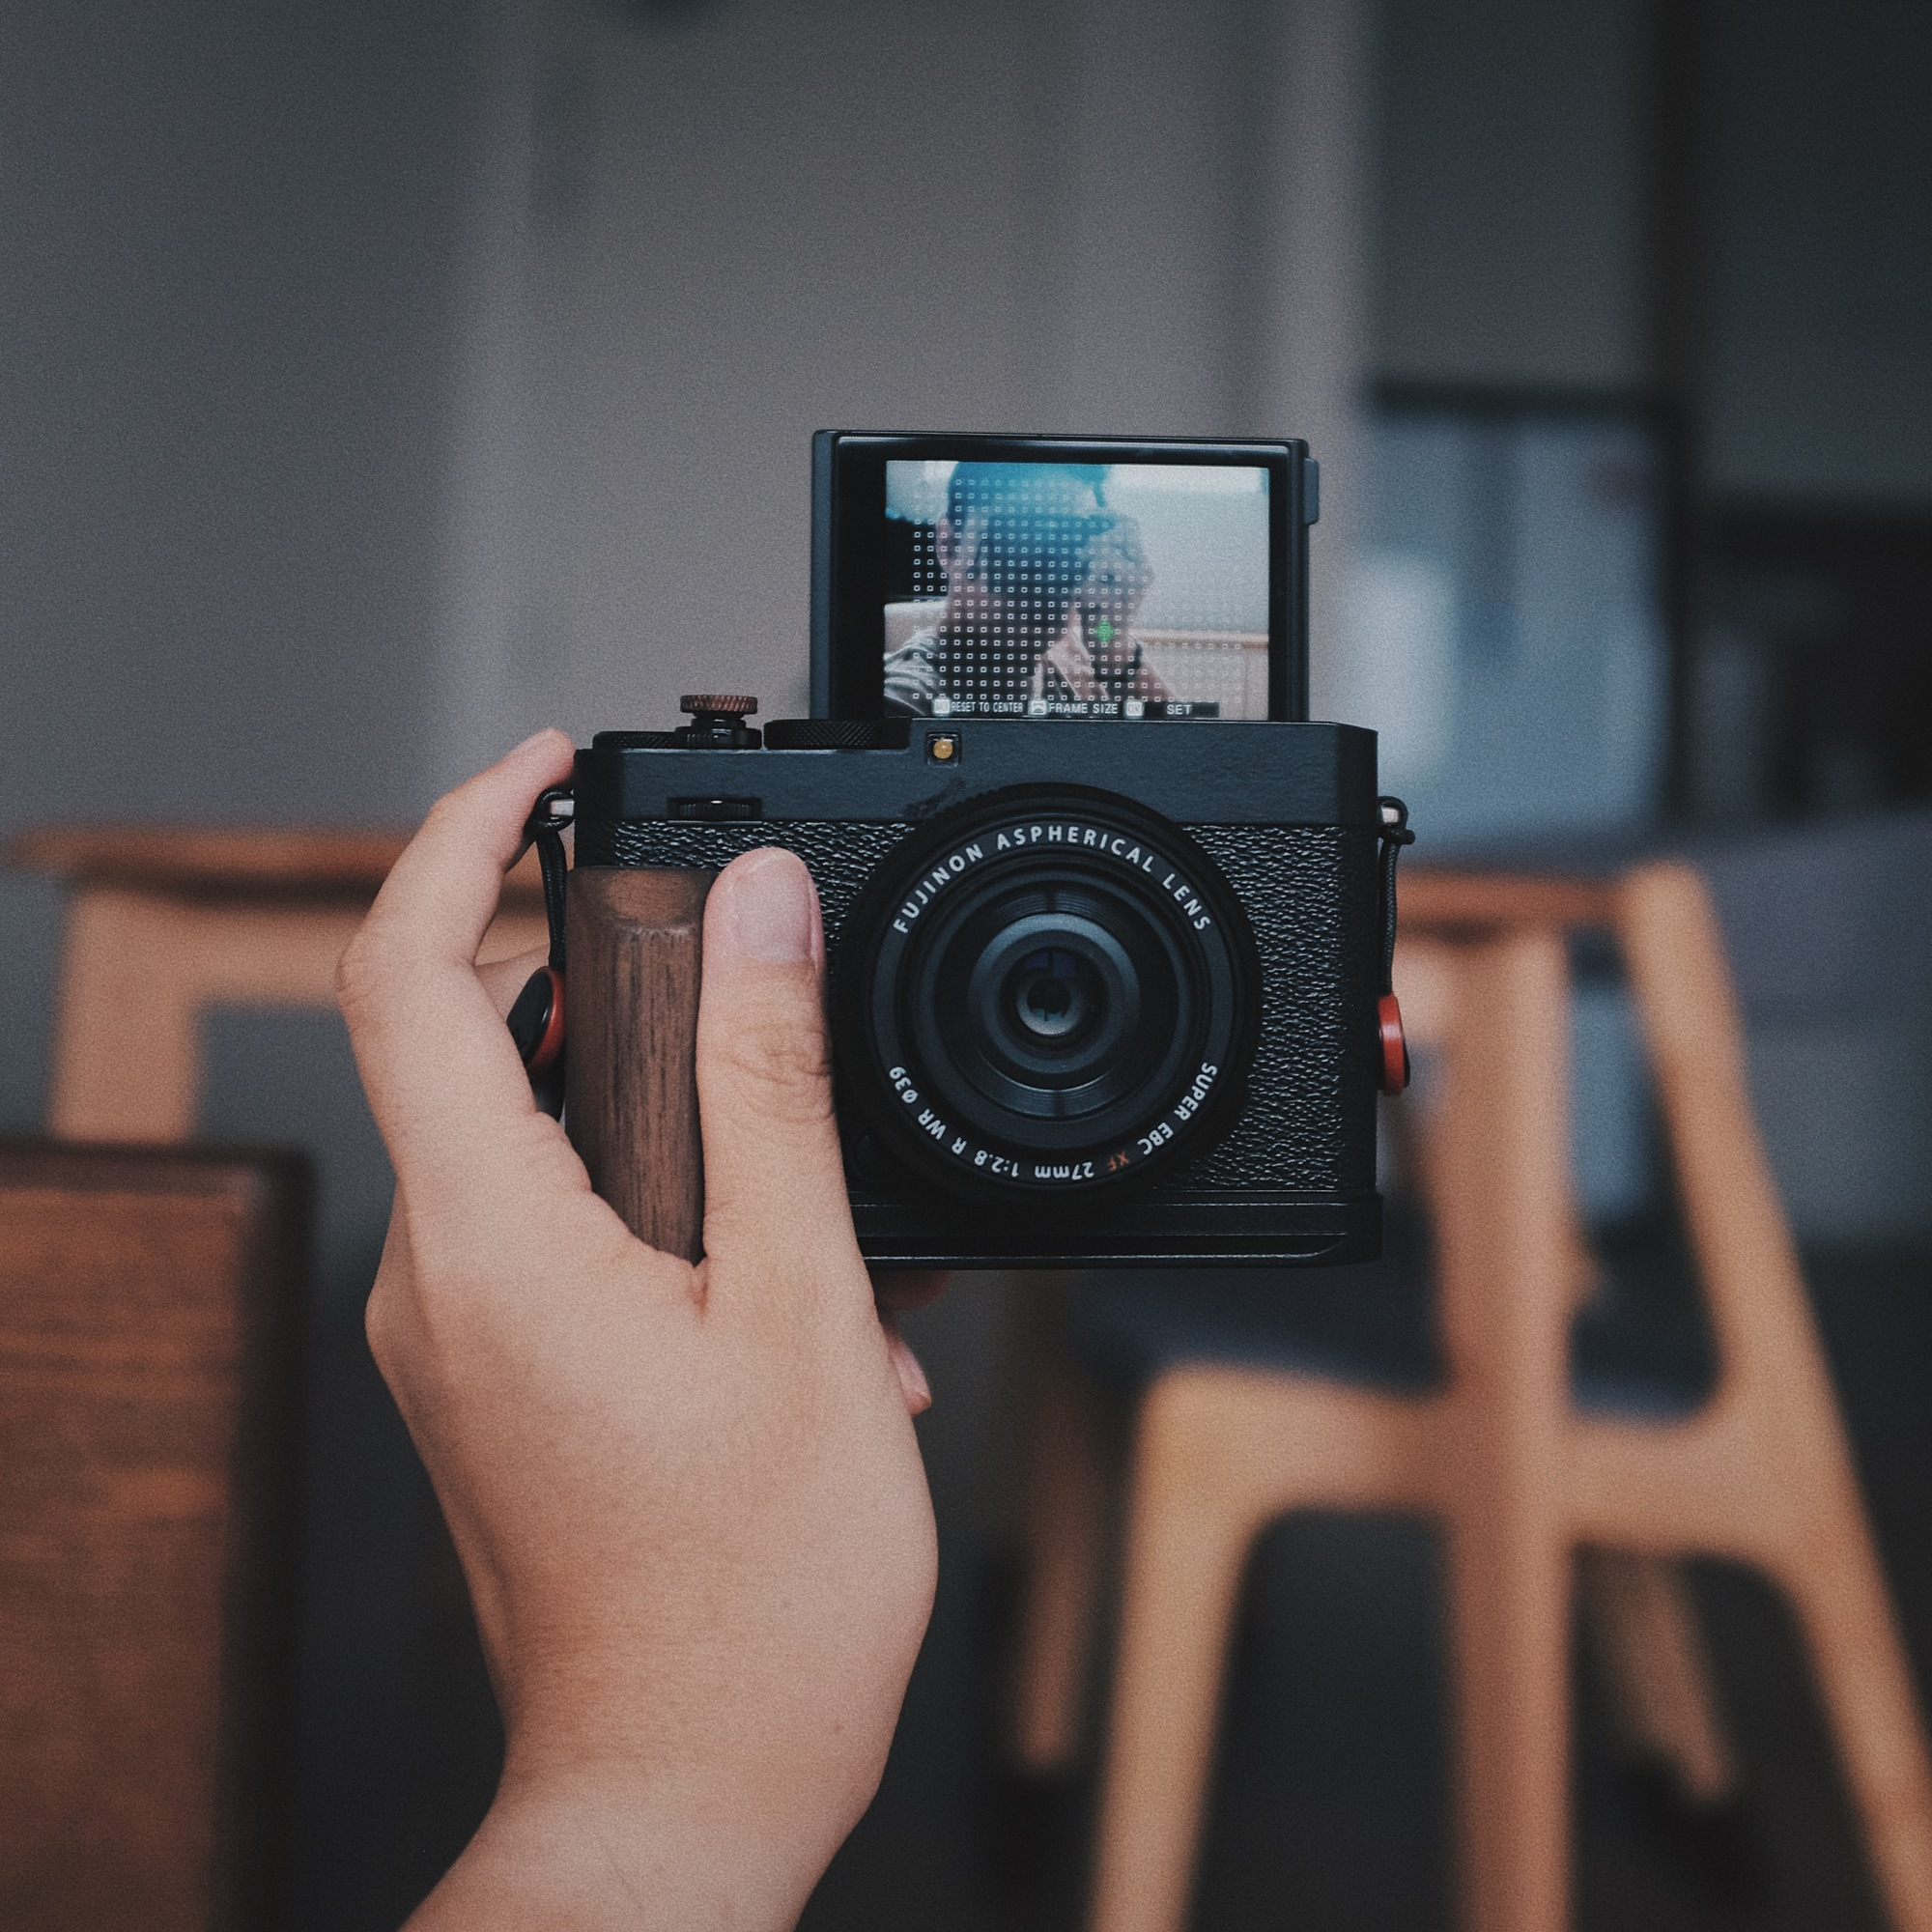
\includegraphics[width=\linewidth]{\envfinaldir/coverpic-prod.jpg}\par
            % \vskip 30pt
            \vfill

            \normalsize\rmfamily\scshape
            \copyright{} The Web Digest Project \hfill\large \envdatestr
        \end{center}
    \end{titlepage}
    % \restoregeometry
}
\newcommand{\simplehref}[1]{%
    \textcolor{blue!80!green}{\href{#1}{#1}}%
}
\renewcommand{\contentsname}{\center\Huge\sffamily\bfseries Contents\par\vskip 20pt}
\newcounter{ipartcounter}
\setcounter{ipartcounter}{0}
\newcommand{\ipart}[1]{
    % \vskip 20pt
    \clearpage
    \stepcounter{ipartcounter}
    \phantomsection
    \addcontentsline{toc}{chapter}{#1}
    % \begin{center}
    %     \Huge
    %     \sffamily\bfseries
    %     #1
    % \end{center}
    % \vskip 20pt plus 7pt
}
\newcounter{ichaptercounter}
\setcounter{ichaptercounter}{0}
\newcommand{\ichapter}[1]{
    % \vskip 20pt
    \clearpage
    \stepcounter{ichaptercounter}
    \phantomsection
    \addcontentsline{toc}{section}{\numberline{\arabic{ichaptercounter}}#1}
    \begin{center}
        \Huge
        \sffamily\bfseries
        #1
    \end{center}
    \vskip 20pt plus 7pt
}
\newcommand{\entrytitlefont}[1]{\subsection*{\raggedright\Large\sffamily\bfseries#1}}
\newcommand{\entryitemGeneric}[2]{
    % argv: title, url
    \parbox{\linewidth}{
        \entrytitlefont{#1}\par\vskip 5pt
        \footnotesize\ttfamily\mdseries
        \simplehref{#2}
    }\vskip 11pt plus 11pt minus 1pt
}
\newcommand{\entryitemGithub}[3]{
    % argv: title, url, desc
    \parbox{\linewidth}{
        \entrytitlefont{#1}\par\vskip 5pt
        \footnotesize\ttfamily\mdseries
        \simplehref{#2}\par\vskip 5pt
        \small\rmfamily\mdseries#3
    }\vskip 11pt plus 11pt minus 1pt
}
\newcommand{\entryitemAp}[3]{
    % argv: title, url, desc
    \parbox{\linewidth}{
        \entrytitlefont{#1}\par\vskip 5pt
        \footnotesize\ttfamily\mdseries
        \simplehref{#2}\par\vskip 5pt
        \small\rmfamily\mdseries#3
    }\vskip 11pt plus 11pt minus 1pt
}
\newcommand{\entryitemHackernews}[3]{
    % argv: title, hnurl, rawurl
    % \parbox{\linewidth}{
    %     \entrytitlefont{#1}\par\vskip 5pt
    %     \footnotesize\ttfamily\mdseries
    %     \simplehref{#3}\par
    %     \textcolor{black!50}{\href{#2}{#2}}
    % }\vskip 11pt plus 11pt minus 1pt
    \begin{minipage}{\linewidth}
            \entrytitlefont{#1}\par\vskip 5pt
            \footnotesize\ttfamily\mdseries
            \simplehref{#3}\par
            \textcolor{black!50}{\href{#2}{#2}}
    \end{minipage}\par\vskip 11pt plus 11pt minus 1pt
}







\begin{document}

\makeheader

\tableofcontents\clearpage




\ipart{Developers}
\ichapter{Hacker News}
\entryitemTwoLinks{Show HN: A minimalist (brutalist?) website for sharing all your links}{https://news.ycombinator.com/item?id=42027654}{https://lynx.boo}

\entryitemTwoLinks{Britain's postwar sugar craze confirms harms of sweet diets in early life}{https://news.ycombinator.com/item?id=42027564}{https://www.science.org/content/article/britain-s-postwar-sugar-craze-confirms-harms-sweet-diets-early-life}

\entryitemTwoLinks{Show HN: Someday, Open-Source Calendly Alternative for Gmail / Google App Script}{https://news.ycombinator.com/item?id=42027187}{https://github.com/rbbydotdev/someday}

\entryitemTwoLinks{Cash: A small jQuery alternative for modern browsers}{https://news.ycombinator.com/item?id=42026054}{https://github.com/fabiospampinato/cash}

\entryitemTwoLinks{Weird Lexical Syntax}{https://news.ycombinator.com/item?id=42024727}{https://justine.lol/lex/}

\entryitemTwoLinks{SmolLM2}{https://news.ycombinator.com/item?id=42024661}{https://simonwillison.net/2024/Nov/2/smollm2/}

\entryitemTwoLinks{Cramming Solitaire onto a Nintendo E-Reader card}{https://news.ycombinator.com/item?id=42024342}{https://mattgreer.dev/blog/cramming-solitaire-onto-a-nintendo-ereader-card/}

\entryitemTwoLinks{Rewrite It in Rails}{https://news.ycombinator.com/item?id=42024246}{https://dirkjonker.bearblog.dev/rewrite-it-in-rails/}

\entryitemTwoLinks{My Time Working at Stripe}{https://news.ycombinator.com/item?id=42023089}{https://jondlm.github.io/website/blog/leaving\_stripe/}

\entryitemTwoLinks{Okta – Username Above 52 Characters Security Advisory}{https://news.ycombinator.com/item?id=42022796}{https://trust.okta.com/security-advisories/okta-ad-ldap-delegated-authentication-username/}

\entryitemTwoLinks{Direct Sockets API in Chrome 131}{https://news.ycombinator.com/item?id=42022649}{https://chromestatus.com/feature/6398297361088512}

\entryitemTwoLinks{Nvidia to join Dow Jones Industrial Average, replacing Intel}{https://news.ycombinator.com/item?id=42022282}{https://www.cnbc.com/2024/11/01/nvidia-to-join-dow-jones-industrial-average-replacing-intel.html}

\entryitemTwoLinks{Sleep regularity is a stronger predictor of mortality than sleep duration (2023)}{https://news.ycombinator.com/item?id=42022151}{https://academic.oup.com/sleep/article/47/1/zsad253/7280269}

\entryitemTwoLinks{Low-cost, portable device can detect colorectal and prostate cancer in an hour}{https://news.ycombinator.com/item?id=42021535}{https://medicalxpress.com/news/2024-10-portable-device-colorectal-prostate-cancer.html}

\entryitemTwoLinks{Linux on Apple Silicon with Alyssa Rosenzweig [audio]}{https://news.ycombinator.com/item?id=42021237}{https://softwareengineeringdaily.com/2024/10/15/linux-apple-silicon-alyssa-rosenzweig/}

\entryitemTwoLinks{Notepad++ is 21 years old}{https://news.ycombinator.com/item?id=42019586}{https://learnhub.top/celebrating-21-years-of-notepad-the-legendary-journey-of-our-favorite-text-editor/}

\entryitemTwoLinks{The Shell Hater's Handbook (2010)}{https://news.ycombinator.com/item?id=42019318}{https://shellhaters.org/talk}

\entryitemTwoLinks{Tell HN: We (Causal) got acquired – thank you HN}{https://news.ycombinator.com/item?id=42019192}{https://news.ycombinator.com/item?id=42019192}

\entryitemTwoLinks{The rise of the U.S., the rise of China}{https://news.ycombinator.com/item?id=42018096}{https://www.construction-physics.com/p/how-china-is-like-the-19th-century}

\entryitemTwoLinks{Apple acquires Pixelmator}{https://news.ycombinator.com/item?id=42018013}{https://www.pixelmator.com/blog/2024/11/01/a-new-home-for-pixelmator/}\ichapter{Phoronix}
\entryitemGeneric{\hskip 0pt{}FreeBSD 14.2 Beta 1 Released To Work Toward This Next Release}{https://www.phoronix.com/news/FreeBSD-14.2-Beta-1-Released}

\entryitemGeneric{\hskip 0pt{}Cloudflare's Pingora 0.4 Rust Framework Released With Experimental Windows Support}{https://www.phoronix.com/news/Cloudflare-Pingora-0.4}

\entryitemGeneric{\hskip 0pt{}Genode-Based Sculpt OS 24.10 Introduces Multi-Monitor Support}{https://www.phoronix.com/news/Genode-Sculpt-OS-24.10}

\entryitemGeneric{\hskip 0pt{}Intel Lands VVC VA-API Hardware Decoding Into FFmpeg}{https://www.phoronix.com/news/VVC-VA-API-FFmpeg-Decode}

\entryitemGeneric{\hskip 0pt{}KDE Will Nicely Notify You When Apps Are Being Killed Due To Out-Of-Memory}{https://www.phoronix.com/news/KDE-Plasma-OOM-Notifications}

\entryitemGeneric{\hskip 0pt{}Vulkan 1.3.301 Released With New Extension For HDR Vivid}{https://www.phoronix.com/news/Vulkan-1.3.301-HDR-Vivid}

\entryitemGeneric{\hskip 0pt{}Xfce 4.20 Pre1 Pre-Release Published For Testing}{https://www.phoronix.com/news/Xfce-4.20-Pre1-Released}

\entryitemGeneric{\hskip 0pt{}Steam On Linux Marketshare Hits 2.0\% For October, AMD CPU Use By Linux Gamers Approaches 75\%}{https://www.phoronix.com/news/Steam-October-2024-Numbers}

\entryitemGeneric{\hskip 0pt{}Wine 10.0 Release Plans Aim For Mid-January Release}{https://www.phoronix.com/news/Wine-10.0-Release-Plans}\ichapter{Dribbble}
\entryitemGeneric{\hskip 0pt{}Lootbox}{https://dribbble.com/shots/24875582}

\entryitemGeneric{\hskip 0pt{}Internal Universe 🪐✨}{https://dribbble.com/shots/24870294}

\entryitemGeneric{\hskip 0pt{}Gulfstream x theory11 Playing Cards}{https://dribbble.com/shots/24869176}

\entryitemGeneric{\hskip 0pt{}Negative yet Positive Vol.7}{https://dribbble.com/shots/24868890}

\entryitemGeneric{\hskip 0pt{}Onton - Responsive Logo Design}{https://dribbble.com/shots/24866015}

\entryitemGeneric{\hskip 0pt{}Solufacil}{https://dribbble.com/shots/24869750}

\entryitemGeneric{\hskip 0pt{}Raw E}{https://dribbble.com/shots/24869489}

\entryitemGeneric{\hskip 0pt{}Ampersand 3D Logo}{https://dribbble.com/shots/24869500}

\entryitemGeneric{\hskip 0pt{}Rooster}{https://dribbble.com/shots/24854380}

\entryitemGeneric{\hskip 0pt{}cipher}{https://dribbble.com/shots/24855823}

\entryitemGeneric{\hskip 0pt{}"Amphiprion Ocellaris" - Daily art, NFT art}{https://dribbble.com/shots/24854577}

\entryitemGeneric{\hskip 0pt{}Bento Cards v.4 – E-Commerce}{https://dribbble.com/shots/24849627}

\entryitemGeneric{\hskip 0pt{}Neobanking Mobile App Interactions}{https://dribbble.com/shots/24848696}

\entryitemGeneric{\hskip 0pt{}FC Shakhtar Donetsk App. The Concept. Part 2}{https://dribbble.com/shots/24848383}

\entryitemGeneric{\hskip 0pt{}xflow Logo Design - X, Waves}{https://dribbble.com/shots/24847689}

\entryitemGeneric{\hskip 0pt{}The Future has landed ✈️}{https://dribbble.com/shots/24848230}

\entryitemGeneric{\hskip 0pt{}Converse Logo Redesign Concept}{https://dribbble.com/shots/24850036}

\entryitemGeneric{\hskip 0pt{}F Logo}{https://dribbble.com/shots/24850079}

\entryitemGeneric{\hskip 0pt{}ML Fashion 10/10}{https://dribbble.com/shots/24851262}

\entryitemGeneric{\hskip 0pt{}Amplemarket Logo Design}{https://dribbble.com/shots/24843224}

\entryitemGeneric{\hskip 0pt{}Streaming Data}{https://dribbble.com/shots/24838862}

\entryitemGeneric{\hskip 0pt{}It's not a feature, it's a bug}{https://dribbble.com/shots/24844082}

\entryitemGeneric{\hskip 0pt{}Cute Raccoon}{https://dribbble.com/shots/24843120}

\entryitemGeneric{\hskip 0pt{}Nero Code UI concept}{https://dribbble.com/shots/24843816}


\ipart{Developers~~~~(zh-Hans)}
\ichapter{Solidot}
\entryitemGeneric{\hskip 0pt{}苹果收购图像编辑应用 Pixelmator}{https://www.solidot.org/story?sid=79664}

\entryitemGeneric{\hskip 0pt{}日本东京高院裁定不承认同性婚姻违宪}{https://www.solidot.org/story?sid=79663}

\entryitemGeneric{\hskip 0pt{}英伟达取代英特尔进入道琼斯工业平均指数}{https://www.solidot.org/story?sid=79662}

\entryitemGeneric{\hskip 0pt{}Linus Torvalds 用电动汽车取代了燃油汽车}{https://www.solidot.org/story?sid=79661}

\entryitemGeneric{\hskip 0pt{}随着减肥药的流行减肥手术减少了四分之一}{https://www.solidot.org/story?sid=79660}

\entryitemGeneric{\hskip 0pt{}蝙蝠仅靠回声可导航数公里}{https://www.solidot.org/story?sid=79659}

\entryitemGeneric{\hskip 0pt{}研究发现猴子永远也写不出莎士比亚著作}{https://www.solidot.org/story?sid=79658}

\entryitemGeneric{\hskip 0pt{}科技行业盛行发布``虚假招聘''}{https://www.solidot.org/story?sid=79657}

\entryitemGeneric{\hskip 0pt{}生命早期限糖可预防成年后罹患糖尿病和高血压}{https://www.solidot.org/story?sid=79656}

\entryitemGeneric{\hskip 0pt{}日本限制边骑车边打手机}{https://www.solidot.org/story?sid=79655}

\entryitemGeneric{\hskip 0pt{}栉水母能逆转衰老}{https://www.solidot.org/story?sid=79654}

\entryitemGeneric{\hskip 0pt{}微软向 Windows 10 用户提供一次性 30 美元的一年安全更新}{https://www.solidot.org/story?sid=79653}

\entryitemGeneric{\hskip 0pt{}Android 16 将于 2025 年二季度发布}{https://www.solidot.org/story?sid=79652}

\entryitemGeneric{\hskip 0pt{}微软再次推迟 Windows Recall}{https://www.solidot.org/story?sid=79651}

\entryitemGeneric{\hskip 0pt{}报告称气候危机导致的高温死亡创下新纪录}{https://www.solidot.org/story?sid=79650}

\entryitemGeneric{\hskip 0pt{}龙芯新处理器据报道性能超过了英特尔的 Raptor Lake}{https://www.solidot.org/story?sid=79649}

\entryitemGeneric{\hskip 0pt{}AMD 宣布 Ryzen 7 9800X3D,售价 479 美元 }{https://www.solidot.org/story?sid=79648}

\entryitemGeneric{\hskip 0pt{}俄罗斯表示计划建立替代 Linux 社区}{https://www.solidot.org/story?sid=79647}

\entryitemGeneric{\hskip 0pt{}瑞典和挪威重新考虑无现金社会计划}{https://www.solidot.org/story?sid=79646}

\entryitemGeneric{\hskip 0pt{}2023 年温室气体浓度创新高}{https://www.solidot.org/story?sid=79645}\ichapter{V2EX}
\entryitemGeneric{\hskip 0pt{}[酷工作] [深圳兼职] 商品验收及物流协调员(细心可靠者优先,无学历要求)}{https://www.v2ex.com/t/1086112}

\entryitemGeneric{\hskip 0pt{}[分享创造] 有没有这样一款产品?(地图相关)}{https://www.v2ex.com/t/1086111}

\entryitemGeneric{\hskip 0pt{}[问与答] 2024 年前三季度结婚登记 474.7 万对,同期减少 94.3 万对,三季度再创单季度新低}{https://www.v2ex.com/t/1086110}

\entryitemGeneric{\hskip 0pt{}[游戏] 英雄联盟 s14}{https://www.v2ex.com/t/1086109}

\entryitemGeneric{\hskip 0pt{}[分享创造] Incredibox Mustard Game Online: incrediboxmustard.cc}{https://www.v2ex.com/t/1086108}

\entryitemGeneric{\hskip 0pt{}[Chrome] Chrome 如何开启自动整理标签页的功能?}{https://www.v2ex.com/t/1086107}

\entryitemGeneric{\hskip 0pt{}[问与答] MacBook pro 是选 m4 32G 还是 m4 pro 24G?}{https://www.v2ex.com/t/1086106}

\entryitemGeneric{\hskip 0pt{}[问与答] 小米 14 保值换新换小米 15,发现屏幕顶部有个黑点}{https://www.v2ex.com/t/1086105}

\entryitemGeneric{\hskip 0pt{}[问与答] 想买点东西,但是不知道买什么}{https://www.v2ex.com/t/1086104}

\entryitemGeneric{\hskip 0pt{}[macOS] 为什么 iPhone 镜像不能用 Mac 的输入法?}{https://www.v2ex.com/t/1086103}

\entryitemGeneric{\hskip 0pt{}[Apple] 8GB 的 MacBook Air M3 和 几年前的 16GB Intel MacBook Pro 相比性能如何?}{https://www.v2ex.com/t/1086102}

\entryitemGeneric{\hskip 0pt{}[宽带症候群] ikuai 如何使用运营商 DNS}{https://www.v2ex.com/t/1086100}

\entryitemGeneric{\hskip 0pt{}[Apple] MacOS 适合作服务器吗?}{https://www.v2ex.com/t/1086099}

\entryitemGeneric{\hskip 0pt{}[MacBook Pro] 都 2025 年了, macbook 这个 sb 刘海遮挡 icon 问题还没有解决}{https://www.v2ex.com/t/1086098}

\entryitemGeneric{\hskip 0pt{}[分享创造] iOS 个人开发者,分享自己开发的两款 APP, AI 绘画:梦幻工坊, ChatGPT 聊天:共鸣 Chat}{https://www.v2ex.com/t/1086097}

\entryitemGeneric{\hskip 0pt{}[Android] magic7pro 和 iqoo13 推荐哪个}{https://www.v2ex.com/t/1086095}

\entryitemGeneric{\hskip 0pt{}[问与答] 米家设备能连上 wifi 但米家不认是什么鬼?}{https://www.v2ex.com/t/1086094}

\entryitemGeneric{\hskip 0pt{}[Android] 安卓小白,想知道国行版的 pad 能刷国际版的 rom 吗?}{https://www.v2ex.com/t/1086092}

\entryitemGeneric{\hskip 0pt{}[宽带症候群] 求小米 AX9000 路由器 iStoreOS 固件}{https://www.v2ex.com/t/1086086}

\entryitemGeneric{\hskip 0pt{}[云计算] 闲置 AWS 和微软证书,需要挂靠联系}{https://www.v2ex.com/t/1086085}

\entryitemGeneric{\hskip 0pt{}[Steam] 如何让 steam 下载彻底不经过 clash}{https://www.v2ex.com/t/1086083}

\entryitemGeneric{\hskip 0pt{}[Windows] 有什么软件可以把手机摄像头通过 USB 来给电脑视频通话使用?}{https://www.v2ex.com/t/1086082}

\entryitemGeneric{\hskip 0pt{}[问与答] 求 1500 以内能用的久点的可以 ROOT 的二手安卓开发机}{https://www.v2ex.com/t/1086080}

\entryitemGeneric{\hskip 0pt{}[iPhone] Another 美区 Apple One Premier 拼车}{https://www.v2ex.com/t/1086079}

\entryitemGeneric{\hskip 0pt{}[iDev] 应该如何推广自己的 APP?}{https://www.v2ex.com/t/1086078}

\entryitemGeneric{\hskip 0pt{}[亚洲] 测试}{https://www.v2ex.com/t/1086077}

\entryitemGeneric{\hskip 0pt{}[Android] 小米终于强兼苹果生态}{https://www.v2ex.com/t/1086076}

\entryitemGeneric{\hskip 0pt{}[Android] 请问一加 13(ColorOS 15)怎么在保持蓝牙打开的前提设置其他设备不可见}{https://www.v2ex.com/t/1086075}

\entryitemGeneric{\hskip 0pt{}[问与答] 有没有什么方法把 quanx 的规则转为 clash 的}{https://www.v2ex.com/t/1086074}

\entryitemGeneric{\hskip 0pt{}[分享创造] 简单写了一个 C++ 的 JSON 库}{https://www.v2ex.com/t/1086073}

\entryitemGeneric{\hskip 0pt{}[生活] 告别舅舅老家}{https://www.v2ex.com/t/1086072}

\entryitemGeneric{\hskip 0pt{}[问与答] 求监控网页变化的软件或开源代码}{https://www.v2ex.com/t/1086071}

\entryitemGeneric{\hskip 0pt{}[问与答] 同一网络下 mac 不能访问路由器管理页,求助}{https://www.v2ex.com/t/1086070}

\entryitemGeneric{\hskip 0pt{}[问与答] 360 极速浏览器不支持手动更新 Widevine 吗}{https://www.v2ex.com/t/1086069}

\entryitemGeneric{\hskip 0pt{}[问与答] Typora 的代码块的行高 怎么调整呀?}{https://www.v2ex.com/t/1086068}

\entryitemGeneric{\hskip 0pt{}[程序员] 网站动态内容太多了, CDN 加速简直就是杯水车薪}{https://www.v2ex.com/t/1086066}

\entryitemGeneric{\hskip 0pt{}[宽带症候群] 7615 买了一年坏掉了...现在有什么便宜的 2.5G 猫推荐吗}{https://www.v2ex.com/t/1086065}

\entryitemGeneric{\hskip 0pt{}[程序员] 从『学习者』『创作者』两个视角,开发了一个开源的 [编程学习] 和 [教程课程搭建] 的工具, 欢迎大家来交流想法}{https://www.v2ex.com/t/1086063}

\entryitemGeneric{\hskip 0pt{}[问与答] 有人试过两台 mac 办公吗}{https://www.v2ex.com/t/1086061}

\entryitemGeneric{\hskip 0pt{}[宽带症候群] WG 回国流量也被墙么?}{https://www.v2ex.com/t/1086060}

\entryitemGeneric{\hskip 0pt{}[DNS] 测试了几家主流 DNS 的 ECS 功能}{https://www.v2ex.com/t/1086059}

\entryitemGeneric{\hskip 0pt{}[程序员] 对于 WebAssembly 2.0 的一些看法}{https://www.v2ex.com/t/1086058}

\entryitemGeneric{\hskip 0pt{}[问与答] 现在有什么好的照片管理工具吗?支持 nas 的,群辉的 photo 好用吗?}{https://www.v2ex.com/t/1086057}

\entryitemGeneric{\hskip 0pt{}[程序员] 真心请教 rk3588 等板子的安卓开发大佬}{https://www.v2ex.com/t/1086056}

\entryitemGeneric{\hskip 0pt{}[京东] 昨天京东给我个 5 元的话费优惠券,然后我充了,今天又自动给我退了。逗我那}{https://www.v2ex.com/t/1086055}

\entryitemGeneric{\hskip 0pt{}[问与答] 现在独立老师这么赚吗?年 50 打底 100 一大排,这比程序员还猛啊!}{https://www.v2ex.com/t/1086054}

\entryitemGeneric{\hskip 0pt{}[京东] 京东真是越来越垃圾了啊}{https://www.v2ex.com/t/1086053}

\entryitemGeneric{\hskip 0pt{}[职场话题] 入职新公司一周,去还是留?}{https://www.v2ex.com/t/1086052}

\entryitemGeneric{\hskip 0pt{}[macOS] surge 体验有感}{https://www.v2ex.com/t/1086051}

\entryitemGeneric{\hskip 0pt{}[分享发现] 小县城真的没钱了}{https://www.v2ex.com/t/1086050}


\ipart{Generic News}
\ichapter{AP News}
\entryitemWithDescription{\hskip 0pt{}TGI Fridays files for bankruptcy protection as sit-down restaurant struggles continue}{https://apnews.com/article/5979e002f72f5595a80d12beee5eeef1}{}

\entryitemWithDescription{\hskip 0pt{}Rohit Bal, one of India's best-known fashion designers, dies at 63}{https://apnews.com/article/1c1843b93ad0b17c572de2dc23449909}{}

\entryitemWithDescription{\hskip 0pt{}Crowds flock to tiny Massachusetts town to send off New York's Rockefeller Christmas tree}{https://apnews.com/article/b61e117d3c93fe1d9d0734e4728eb77c}{}

\entryitemWithDescription{\hskip 0pt{}Shark bites 61-year-old Maui surfer, completely severing his leg below the knee}{https://apnews.com/article/f2cab9b0c84d27a841dd0aa8e4f034e7}{}

\entryitemWithDescription{\hskip 0pt{}Meet Decoy Ohtani, perhaps the most valuable pet of the World Series}{https://apnews.com/article/a14dfd0faae2aad9cfd557ebc89638f7}{}

\entryitemWithDescription{\hskip 0pt{}Daylight saving time ends Sunday. Time to `fall back' an hour}{https://apnews.com/article/251e55ce23d25a490783a996915dbc22}{}

\entryitemWithDescription{\hskip 0pt{}Wendy's closing 140 more restaurants}{https://apnews.com/article/69c3b496b3038f9f03bcbbae231a0e64}{}

\entryitemWithDescription{\hskip 0pt{}`Amateurish' thieves steal 2 Warhol prints, damage 2 more in botched heist at Dutch gallery}{https://apnews.com/article/6d45495ea8b48c9ab09379eed28c19f1}{}

\entryitemWithDescription{\hskip 0pt{}Macy's Thanksgiving Parade will feature Ariana Madix, T-Pain, `Gabby's Dollhouse' and pasta}{https://apnews.com/article/a9296caedf1cfed0f29ad5ce1bfaaec5}{}

\entryitemWithDescription{\hskip 0pt{}Not just for summer: `Brat' is Collins Dictionary's word of the year}{https://apnews.com/article/c495163b1562bd72f611192ddc5da3c2}{}

\entryitemWithDescription{\hskip 0pt{}Deaths of 10 newborns shake millions' trust in Turkey's health care system}{https://apnews.com/article/d99b0e3bb58295b4dc31e9b44fd49201}{}

\entryitemWithDescription{\hskip 0pt{}We are what we celebrate: America's holiday calendar is increasingly diverse}{https://apnews.com/article/d258c1f6078af76a8eec487a583f90d2}{}

\entryitemWithDescription{\hskip 0pt{}Heidi Klum and Janelle Monáe wear E.T. costumes for their Halloween parties}{https://apnews.com/article/2bb5c6f8b6c34c187a8fd63b36ddcda3}{}\ichapter{Reuters}
\entryitemWithDescription{\hskip 0pt{}Israeli military says it killed Hezbollah unit commander in southern Lebanon}{https://www.reuters.com/world/middle-east/israeli-military-says-it-killed-hezbollah-unit-commander-southern-lebanon-2024-11-02/}{The Israeli military said on Saturday it had killed Jaafar Khader Faour, a commander of Hezbollah\textquotesingle s Nasser Brigade rocket unit in southern Lebanon, and said he had been responsible for multiple attacks on Israel since...}

\entryitemWithDescription{\hskip 0pt{}Israel eases restrictions in north amid heightened tensions with Hezbollah}{https://www.reuters.com/world/middle-east/israel-eases-restrictions-north-amid-heightened-tensions-with-hezbollah-2024-11-02/}{Israel\textquotesingle s military announced updates to its Home Front Command\textquotesingle s defensive guidelines on Saturday, raising the alert level in the Lower Galilee and southern Golan regions from "partial" to "...}

\entryitemWithDescription{\hskip 0pt{}Woman strips off clothes at Iran university in apparent protest, reports say}{https://www.reuters.com/world/middle-east/woman-strips-off-clothes-iran-university-apparent-protest-reports-say-2024-11-02/}{A young woman stripped to her underwear at an Iranian university on Saturday in an apparent protest against the country\textquotesingle s strict Islamic dress code, according to online videos and media...}

\entryitemWithDescription{\hskip 0pt{}Egypt hosts Fatah-Hamas post-war Gaza talks as part of ceasefire efforts}{https://www.reuters.com/world/middle-east/egypt-hosts-fatah-hamas-post-war-gaza-talks-part-ceasefire-efforts-2024-11-02/}{Senior officials of the rival Palestinian groups Fatah and Hamas are meeting in Cairo to discuss forming a committee to manage Gaza\textquotesingle s post-war governance, an Egyptian security source was quoted as saying by Egypt...}

\entryitemWithDescription{\hskip 0pt{}Austrian president to have spinal surgery, chancellor to stand in}{https://www.reuters.com/world/europe/austrian-president-have-spinal-surgery-chancellor-stand-2024-11-02/}{Austria\textquotesingle s President Alexander Van der Bellen, who is overseeing coalition talks following the country\textquotesingle s recent election, will undergo spinal surgery, his office said on...}

\entryitemWithDescription{\hskip 0pt{}FBI dismisses video claiming it apprehended groups committing ballot fraud}{https://www.reuters.com/world/us/fbi-dismisses-video-claiming-it-apprehended-groups-committing-ballot-fraud-2024-11-02/}{The FBI said on Saturday that a video claiming it had apprehended three linked groups committing ballot fraud and another related to Democratic presidential candidate Kamala Harris\textquotesingle{} husband are not...}

\entryitemWithDescription{\hskip 0pt{}Russia says Ukraine is sabotaging prisoner of war exchanges}{https://www.reuters.com/world/europe/russia-says-ukraine-is-sabotaging-prisoner-war-exchanges-2024-11-02/}{Russian Foreign Ministry spokeswoman Maria Zakharova said on Saturday that Ukraine was essentially sabotaging the process of exchanging prisoners of...}

\entryitemWithDescription{\hskip 0pt{}Israeli naval force detains person after landing in Lebanese coastal town, sources say}{https://www.reuters.com/world/middle-east/israeli-forces-land-lebanese-coastal-town-seize-one-person-sources-say-2024-11-02/}{An Israeli military official said a senior Hezbollah operative was...}

\entryitemWithDescription{\hskip 0pt{}US citizen who helped Russia from Ukraine appears in Moscow}{https://www.reuters.com/world/us-citizen-who-helped-russia-ukraine-appears-moscow-2024-11-02/}{A U.S. citizen who was spirited out of eastern Ukraine by Russian special forces after helping the Kremlin target Ukrainian troops said in Moscow on Saturday he had asked for Russian...}

\entryitemWithDescription{\hskip 0pt{}India criticises Canada for linking minister to Sikh plots}{https://www.reuters.com/world/india/india-slams-canada-linking-home-minister-sikh-plots-2024-11-02/}{India\textquotesingle s foreign ministry said on Saturday it had lodged a protest with Canada for linking its home minister to alleged plots against Sikh separatists on Canadian...}

\entryitemWithDescription{\hskip 0pt{}Who is Kemi Badenoch, the UK Conservatives' new leader?}{https://www.reuters.com/world/uk/combative-badenoch-steer-uk-conservatives-towards-populist-right-2024-11-02/}{The self-proclaimed straight speaker will bring a right-wing tone to the...}

\entryitemWithDescription{\hskip 0pt{}Serbia probes fatal train station roof collapse as vigil held for victims}{https://www.reuters.com/world/europe/serbia-opens-probe-into-railway-building-disaster-that-killed-14-2024-11-02/}{Serbia wound up a rescue operation and opened an investigation on Saturday into a roof collapse at a railway station in the northern city of Novi Sad that killed 14 people and injured three...}

\entryitemWithDescription{\hskip 0pt{}Spain mounts biggest peacetime disaster recovery operation as death toll reaches 211}{https://www.reuters.com/world/europe/thousands-join-effort-clean-up-catastrophic-spanish-floods-2024-11-02/}{The tragedy is already Europe\textquotesingle s worst flood-related disaster since 1967 when at least 500 people died in...}






\clearpage
\leavevmode\vfill
\footnotesize

Copyright \copyright{} 2023-2024 Neruthes and other contributors.

This document is published with CC BY-NC-ND 4.0 license.

The entries listed in this newsletter may be copyrighted by their respective creators.

This newsletter is generated by the Web Digest project.

The newsletters are also delivered via Telegram channel \CJKunderline{\href{https://t.me/webdigestchannel}{https://t.me/webdigestchannel}}.\\
RSS feed is available at \CJKunderline{\href{https://webdigest.pages.dev/rss.xml}{https://webdigest.pages.dev/rss.xml}}.

This newsletter is available in PDF at
\CJKunderline{\href{https://webdigest.pages.dev/}{https://webdigest.pages.dev/}}.

The source code being used to generate this newsletter is available at\\
\CJKunderline{\href{https://github.com/neruthes/webdigest}{https://github.com/neruthes/webdigest}}.

This newsletter is also available in
\CJKunderline{\href{http://webdigest.pages.dev/readhtml/\envyear/WebDigest-20241103.html}{HTML}} and
\CJKunderline{\href{https://github.com/neruthes/webdigest/blob/master/markdown/\envyear/WebDigest-20241103.md}{Markdown}}.


\coverpic{https://unsplash.com/photos/a-couch-and-table-in-a-small-room-WvSeZ3rQn0E}{Lena Polishko}


\end{document}
